\documentclass[10pt]{exam}

\usepackage[margin=1in]{geometry}
\usepackage{amsmath}
\usepackage{amssymb}
\usepackage{amsthm}
\usepackage{mathtools}
\usepackage{bm}

\usepackage{color}
\usepackage{colortbl}
\definecolor{deepblue}{rgb}{0,0,0.5}
\definecolor{deepred}{rgb}{0.6,0,0}
\definecolor{deepgreen}{rgb}{0,0.5,0}
\definecolor{gray}{rgb}{0.7,0.7,0.7}

\usepackage{hyperref}
\hypersetup{
  colorlinks   = true, %Colours links instead of ugly boxes
  urlcolor     = black, %Colour for external hyperlinks
  linkcolor    = blue, %Colour of internal links
  citecolor    = blue  %Colour of citations
}

%%%%%%%%%%%%%%%%%%%%%%%%%%%%%%%%%%%%%%%%%%%%%%%%%%%%%%%%%%%%%%%%%%%%%%%%%%%%%%%%

\newcommand*{\hl}[1]{\colorbox{yellow}{#1}}

\newcommand*{\answerLong}[2]{
    \ifprintanswers{\hl{#1}}
\else{#2}
\fi
}

\newcommand*{\answer}[1]{\answerLong{#1}{~}}

\newcommand*{\TrueFalse}[1]{%
\ifprintanswers
    \ifthenelse{\equal{#1}{T}}{%
        \hl{\textbf{TRUE}}\hspace*{14pt}False
    }{
        True\hspace*{14pt}\hl{\textbf{FALSE}}
    }
\else
    \texttt{True}\hspace*{20pt}\texttt{False}\hspace*{20pt}\texttt{Open}
\fi
} 
%% The following code is based on an answer by Gonzalo Medina
%% https://tex.stackexchange.com/a/13106/39194
\newlength\TFlengthA
\newlength\TFlengthB
\settowidth\TFlengthA{\hspace*{1.8in}}
\newcommand\TFQuestion[2]{%
    \setlength\TFlengthB{\linewidth}
    \addtolength\TFlengthB{-\TFlengthA}
    \noindent
    \parbox[t]{\TFlengthA}{\TrueFalse{#1}}\parbox[t]{\TFlengthB}{#2}
    \vspace{0.25in}
}

%%%%%%%%%%%%%%%%%%%%%%%%%%%%%%%%%%%%%%%%%%%%%%%%%%%%%%%%%%%%%%%%%%%%%%%%%%%%%%%%

\theoremstyle{definition}
\newtheorem{problem}{Problem}
\newtheorem{theorem}{Theorem}
\newtheorem{defn}{Definition}
\newtheorem{refr}{References}
\newcommand{\E}{\mathbb E}
\newcommand{\R}{\mathbb R}
\DeclareMathOperator{\nnz}{nnz}
\DeclareMathOperator{\determinant}{det}
\DeclareMathOperator{\Var}{Var}
\DeclareMathOperator{\rank}{rank}
\DeclareMathOperator*{\argmin}{arg\,min}
\DeclareMathOperator*{\argmax}{arg\,max}

\newcommand{\I}{\mathbf I}
\newcommand{\Q}{\mathbf Q}
\newcommand{\p}{\mathbf P}
\newcommand{\pb}{\bar {\p}}
\newcommand{\pbb}{\bar {\pb}}
\newcommand{\pr}{\bm \pi}

\newcommand{\trans}[1]{{#1}^{T}}
\newcommand{\loss}{\ell}
\newcommand{\w}{\mathbf w}
\newcommand{\x}{\mathbf x}
\newcommand{\y}{\mathbf y}
\newcommand{\lone}[1]{{\lVert {#1} \rVert}_1}
\newcommand{\ltwo}[1]{{\lVert {#1} \rVert}_2}
\newcommand{\lp}[1]{{\lVert {#1} \rVert}_p}
\newcommand{\linf}[1]{{\lVert {#1} \rVert}_\infty}
\newcommand{\lF}[1]{{\lVert {#1} \rVert}_F}

\newcommand{\ignore}[1]{}

%%%%%%%%%%%%%%%%%%%%%%%%%%%%%%%%%%%%%%%%%%%%%%%%%%%%%%%%%%%%%%%%%%%%%%%%%%%%%%%%

\begin{document}


\begin{center}
{
\Huge
    Notes: Pagerank III (the last one!)
}

\vspace{0.15in}
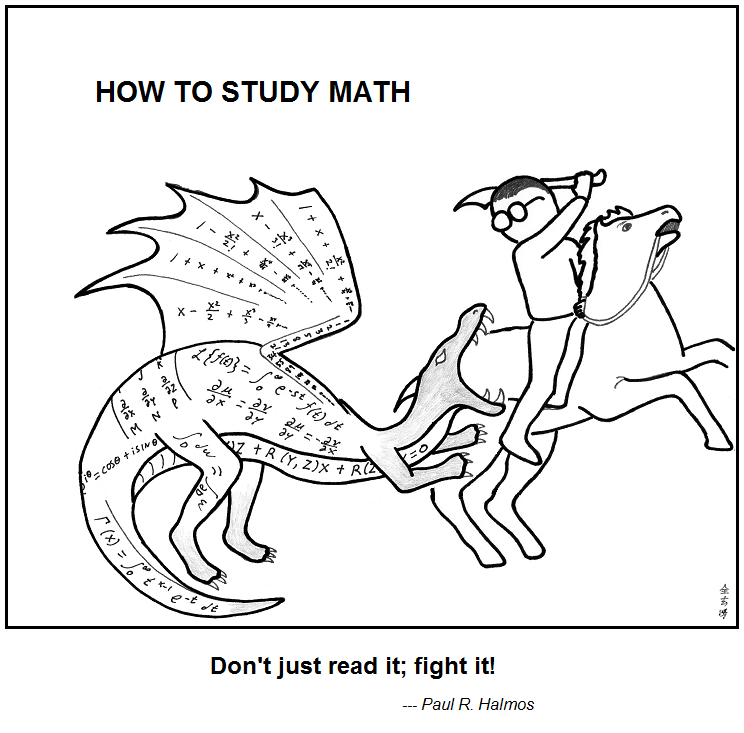
\includegraphics[width=3in]{saint_curious_george}
\vspace{-0.15in}

%Due: Sunday, 6 Sep 2020 at midnight
\end{center}

\begin{center}
%
\includegraphics[width=\textwidth]{dilbert}
\end{center}

\section{Alternative Motivations}

Pagerank can be used in many situations besides web ranking.
In particular, if you can formalize your problem as somehow finding the ``most important'' nodes in a graph where something important is ``flowing'' between those nodes,
then you can use pagerank.

\begin{problem}
    Describe how pagerank can be used for the following tasks.
    \begin{enumerate}
        \item 
            You are in charge of advertising the new Apple iGadget.
            You want to deliver free samples to Twitter influencers,
            with the hope that they will write good reviews that cause many people to purchase the iGadget.
            How do you select which people to give these free samples to?
            \newpage
        \item 
            You are the director of the CIA and you want to kill terrorists.
            How do you identify likely terrorists?


            \vspace{8in}
            NOTE:
            In 2014, former CIA and NSA director Michael Hayden famously said ``We kill people based on metadata.''
            This is exactly what he was referring to.
            See:

            %\begin{quote}
            \url{https://www.justsecurity.org/10318/video-clip-director-nsa-cia-we-kill-people-based-metadata/}
            %\end{quote}
    \end{enumerate}
\end{problem}

\newpage
\begin{problem}
    Create an example problem statement similar to the problem statements from Problem 1 above,
    and describe how the problem can be solved using pagerank.
\end{problem}

%\newpage
%\begin{problem}
    %Describe a graph problem where it would NOT make sense to use pagerank.
%\end{problem}

%\newpage
%\section{Alternative Analysis}
%
%\begin{problem}
    %Previously, we analyzed the pagerank algorithm in terms of the residual $\ltwo{\x^{(K)} - \x^{(K-1}}$ since that is how the analysis was presented in the paper.
    %A slightly more powerful analysis is to directly measure the error of our algorithm
%\end{problem}

\newpage
\section{A Faster Algorithm?}

\begin{problem}
    There are many algorithms for computing top eigenvectors,
    and any of these algorithms can be used to compute the pagerank vector.
    In this problem, we will investigate the \emph{exponentially accelerated power method} (EAPM).
    The EAPM a divide and conquer algorithm that can achieve the same accuracy $\epsilon$ as the power method with only a logarithmic number of iterations.

    The EAPM does not have a standard name,
    and so it is not something you can easily google to learn more about.
    Furthermore, it is not covered in the reference paper.
    Therefore, you will have to solve all of the problems below on your own without aide from outside sources.
    The surface-level purpose of this problem is to get you to understand the EAPM trick,
    but the deeper purpose of this problem is to get you comfortable analyzing algorithms for which there is no reference analysis available anywhere in the world.

    Recall that in the standard power method, at each iteration we perform the computation in Eq (5.1) from the text.
    It is reproduced below:
    \begin{equation}
        \label{eq:pbb}
        \x^{(K)T} = {\x^{(K-1)T}} \pbb
        .
    \end{equation}
    Unraveling the recursion, we have that
    \begin{equation}
        \label{eq:pbbk}
        \x^{(K)T} = {\x^{(0)T}} \pbb^K
        .
    \end{equation}
    In the standard power method, we solve Eq \eqref{eq:pbbk} with a procedure involving $K$ matrix-vector operations.
    The key idea of the EAPM is to ``reparenthesize'' these operations to instead solve $\log K$ matrix-matrix operations.
    We will see that in some cases this reparenthesization results in much (i.e. exponentially) faster runtimes.


    The output of the EAPM after $K$ iterations is the vector $\y^{(K)}$, which is defined as
    \begin{equation}
        \label{eq:exp:y}
        \y^{(K)} = \frac{\x^{(0)T} \Q_K}{\ltwo{\x^{(0)T} \Q_K}}
        ,
    \end{equation}
    where
    \begin{equation}
        \label{eq:Qk}
        \Q_K = 
        \begin{cases}
            \pbb & \text{if}~K=0 \\
            \Q_{K-1} \Q_{K-1} & \text{otherwise} \\
        \end{cases}
        .
    \end{equation}
    In the standard power method, the matrix $\pbb$ is not stored explicitly;
    we substitute the definition of $\pbb$ into Eq \eqref{eq:pbb} above and perform all calculations on the sparse $\p$ matrix.
    In the EAPM, the $\pbb$ matrix is stored explicitly as a dense matrix,
    and each $\Q_K$ is also stored as a dense matrix.

    \begin{enumerate}
        %\item
            %Show that $\y^{(K)} = \x^{(2^K)}$.
            %This equivalence is why the algorithm is ``exponentially accelerated.''
%
            %HINT: 
            %Use induction to show that $Q_{K} = \pbb^{2^{K}}$.
            %The result follows by combining this fact with \eqref{eq:exp:y} and Equation (5.1) in the paper.
            %\vspace{3in}

        \newpage
        \item
            What is the runtime of calculating $\Q_K$ given $\Q_{K-1}$? 
            \vspace{4in}

        \item 
            What is the runtime of computing $\y^{(K)}$ in terms of $K$?
            \vspace{3in}

        \newpage
        \item
            As with the standard power method, we do not know the total number of iterations of the exponential power method in advance.
            Instead, we iterate until the answer is ``good enough'' as measured by the residual.
            That is, we iterate until
            %For this problem, we will directly compare the distance between the $K$th iterate to the unknown pagerank vector,
            %and iterate until the following condition is satisfied:
            \begin{equation}
                \label{eq:exp:eps}
                \ltwo{\y^{(K)}-\y^{(K-1)}} \le \epsilon,
            \end{equation}
            where $\epsilon$ is a predetermined small constant value.
            The \emph{Deeper Inside Pagerank} paper does not discuss the EAPM algorithm, so I have provided below a simple theorem (without proof) about its convergence rate.
            \begin{theorem}
                \label{thm:EAPM}
                For all $K$, the EAPM satisfies
                \begin{equation}
                    \ltwo{\y^{(K)}-\y^{(K-1)}} \le \alpha^{2^K}.
                \end{equation}
            \end{theorem}
            %\begin{proof}
            %\begin{align}
                %\ltwo{\y^{(K)} - \y^{(K-1)}}
                %&= \ltwo{\x^{(2^K)} - \x^{2^{K-1}}} \\
                %&= \ltwo{\sum_{i=2^{K-1}}^{2^K - 1} (\x^{(i+1)} - \x^{(i)})} \\
                %&\le \sum_{i=2^{K-1}}^{2^K - 1} \ltwo{(\x^{(i+1)} - \x^{(i)})} \\
                %&\le \sum_{i=2^{K-1}}^{2^K - 1} \alpha^i \\
                %&\le 2^{K-1} \alpha^{2^{K-1}} \\
                %%&\le \alpha^{2^{K-2}}
                %%&= O\bigg(\alpha^{2^{K-2}} \bigg)
                %&\le 2^{K-1} \alpha^{2^{K-1}} \\
                %\label{eq:exp:align}
            %\end{align}
            %\end{proof}

            Use Theorem \ref{thm:EAPM} above to compute the number of iterations $K$ required to achieve a target $\epsilon$ value.
            %Bounding the number of iterations $K$ required to satisfy \eqref{eq:exp:eps} is a bit more technical than in the previous problem.
            %You do not have to compute a bound on $K$ yourself,
            %and may instead assume that 
            %\begin{equation}
                %\label{eq:exp:2}
                %K = O\bigg( \log \frac{\log \epsilon}{\log \alpha} \bigg)
            %\end{equation}
            %satisfies \eqref{eq:exp:eps}.
            %Notice that this number of iterations is logrithmic compared to the number of iterations in the standard power method,
            %and this is where the name exponentially accelerated comes from.

            %%You do not need to understand the technical details of the proof of \eqref{eq:exp:2},
            %%but it is reproduced below for the curious.
            %\begin{align}
                %\ltwo{\y^{(K)} - \y^{(K-1)}}
                %&= \ltwo{\x^{(2^K)} - \x^{2^{K-1}}} \\
                %&= \ltwo{\sum_{i=2^{K-1}}^{2^K - 1} (\x^{(i+1)} - \x^{(i)})} \\
                %&\le \sum_{i=2^{K-1}}^{2^K - 1} \ltwo{(\x^{(i+1)} - \x^{(i)})} \\
                %&\le \sum_{i=2^{K-1}}^{2^K - 1} \alpha^i \\
                %&\le 2^{K-1} \alpha^{2^{K-1}} \\
                %%&\le \alpha^{2^{K-2}}
                %&= O\bigg(\alpha^{2^{K-2}} \bigg)
                %\label{eq:exp:align}
            %\end{align}
            %Next, we set the right hand side of \eqref{eq:exp:align} less than $\epsilon$,
            %and solve for $K$.
            %\begin{align}
                %\alpha^{2^{K-2}} &\le \epsilon \\
                %{2^{K-2}}\log \alpha &\le \log \epsilon \\
                %{2^{K-2}} &\ge \frac{\log \epsilon}{\log \alpha} \\
                %K-2 & \ge \log_2\frac{\log \epsilon}{\log \alpha} \\
                %K & \ge 2 + \log_2\frac{\log \epsilon}{\log \alpha} \\
                %K & = O\bigg(\log \frac{\log\epsilon}{\log \alpha} \bigg) 
            %\end{align}

        %\item

            \vspace{3.5in}
        \item
            What is the runtime of computing $\y^{(K)}$ in terms of $\epsilon$?
            \vspace{4.5in}

        \newpage
        \item
            Under what conditions is the exponentially accelerated power method faster or slower than the standard power method?
            \vspace{4in}

        %\item
            %Under what conditions is it slower?
            %\vspace{3in}

        %\newpage
        \item
            Why does it not make sense to use the exponentially accelerated power method to compute the pagerank vector?
            In particular, what bad thing(s) would happen if $\p$ was stored as a sparse matrix, and we substitute the defintion of $\pbb$ in terms of $\p$ into Eq \ref{eq:Qk} above?
            \vspace{4in}
%
    \end{enumerate}
\end{problem}

\end{document}



